% There are two otion that can be provided to the uofathesis class
% 1) published - adjusts the declaration to include a statement regarding published materials. This is required if any chapters in your thesis have been published.
% 2) international - include this if you are an international student to exclude the paragraph regarding the Australian Government Research Training Program Scholarship 
\documentclass[published]{uofathesis}

% Any packages should go here
\usepackage{lineno,setspace}
\usepackage{caption}
\usepackage{booktabs}
\usepackage{amsmath,amssymb,amsfonts,amsbsy}
\usepackage{rotating,array,multirow}
\usepackage{textcomp}
\usepackage{afterpage, emptypage}
\usepackage{pdflscape}
\usepackage{graphicx,natbib} 
\usepackage{hyperref}
\usepackage{geometry}
\usepackage{layouts}
\usepackage{pdfpages}
\usepackage{epigraph} 
\usepackage{xcolor}
\usepackage{listings}
\usepackage{tikz}
\usetikzlibrary{shapes.geometric}
\usetikzlibrary{quotes,angles}
\usepackage{tikz}
\usetikzlibrary{decorations.pathmorphing,patterns}
\usetikzlibrary{shapes.geometric, arrows}
\tikzstyle{startstop} = [rectangle, rounded corners, minimum width=3cm, minimum height=1cm,text centered, draw=black, fill=red!30]
\tikzstyle{io} = [trapezium, trapezium left angle=70, trapezium right angle=110, minimum width=3cm, minimum height=1cm, text centered, draw=black, fill=blue!30]
\tikzstyle{process} = [rectangle, minimum width=3cm, minimum height=1cm, text centered, draw=black, fill=orange!30]
\tikzstyle{decision} = [diamond, minimum width=3cm, minimum height=1cm, text centered, draw=black, fill=green!30]
\tikzstyle{arrow} = [thick,->,>=stealth]
\usetikzlibrary{shapes.multipart}
\usetikzlibrary{positioning}
\usepackage{pgfplots}
\pgfplotsset{compat = newest}
\usepackage{array}








\usepackage{url}
\usepackage{physics}
\usepackage{matlab-prettifier}




\usepackage{xparse}

\NewDocumentCommand{\codeword}{v}{%
\texttt{\textcolor{blue}{#1}}%
}


\usepackage[titletoc,toc,page]{appendix}
\usepackage{lipsum}
\renewcommand{\appendixpagename}{\appendixname}

\renewcommand{\appendixtocname}{\appendixname}

\noappendicestocpagenum



% SET MARGINS
\geometry{outer=20mm,inner=35mm}

% ADD HYPERLINKS TO DOCUMENT BUT MAINTAIN BLACK FONT
\hypersetup{colorlinks=true,allcolors=}

\title{An Off-lattice Computational Model for the Growth of Saccharomyces Cerevisiae}
\titlesize{\huge} % recommend using any of \large, \Large, \LARGE, \huge, \HUGE, depening on length of title. 
\author{Isaac Nakone}
\degree{Bachelor of Mathematical Sciences - Honours}
\department{School of Computer and Mathematical Sciences}
\school{Faculty of Sciences, Engineering and Technology}

% PATHS TO FIGURES - add these as needed
\graphicspath{
    {chapter1/figures/}
    {chapter2/figures/}
    }

% Use the includeonly command to work on individual chapters at a time.
% Comment out this command to build the entire document.
% \includeonly{chapter1/body}

\begin{document}
\frontmatter
\maketitle

% Create the following tables
\tableofcontents
\listoftables
\listoffigures

% HDR Declaration
\makedeclaration

% Import the various things
\chapter{Acknowledgements}

\textit{Where to begin?}
\\
Thank you to my supervisers, Ed Green and Sanjeeva Balasuriya,
for your enduring support during these \textit{two and a half} 
years.
\\
Thankyou to my highschool English teacher, Tanja, for teaching
me how to use form and technique in my writing.
\\
Thank you to my parents, Debbie and Alex, and to my sister,
Amelia. In your own way, you each provided the soil 
from which this thesis grew.
\\
Thank you to my literary friend, John, whose cerebral writing 
will have inspired a generation of \textit{rebels with a cause} by 
next Tuesday, I'm sure of it.
\\
Thank you to Ki and my other colleagues at \textit{Adelaide University}
for providing the environmental stresses to keep me growing. Ki 
was always willing to speak with me and offer his time. 
I am grateful.
\\
There appears to be a collection of \textit{Alex}'s in my life.
I thank you all dearly in one foul sweep. 
\\
To \textit{Radee}, for reminding be how to thinking critically 
and creatively at the same time.
\\
To Harry and Zehao and the other engineers one of whom is another \textit{Alex},
I appreciate you.
\\
To Giuseppe, thank you for introducing me to the \textit{bible of statistical mechanics}.
\\
For the fruitful \textit{Kong-Tchorbadjiev-Nakone} (KTN) correspondence,
for your years of philosphical musing.
\\
Thank you to \textit{cafe} staff at the university for your 
unassuming presence among the day-to-day emergence of new forms.
\\
Thankyou to the late philosophy Professor Michael Sugrue,
whose lectures, both young and old, were stunning depictions
of daring heart of philosophy.
\\
Thankyou to \textit{ChatGPT},
for helping me externalise my interior geometry.
It materialised in the form of the great parable of baker's yeast.
\\
If there was anyone I forgot, I hope you are not offended.
\\

\textit{Isaac}

\chapter{Abstract}
Baker's yeast (\textit{Saccharomyces cerevisiae}) is capable 
of undergoing a pseudohyphal transition to filamentous growth in nutrient poor environments.
An algebraic representation of \textit{S. cerevisiae} cells is adapted from
computer graphics to model cellular division (mitosis) at low computational cost.
By reimagining mitosis as topological bifurcation using level sections 
of signed distance functions (SDFs) underpinned by a discrete mechanistic network, 
novel predictions about 
\textit{S. cerevisiae} colony morphology are made. Coupling 
the algbraic biomass field to a traditional reaction diffusion system 
for nutrient allows the relationship between metabolism 
and growth rate to be estimated for this agent based 
model (ABM). A measure for filamentous branching called compactness 
is introduced and related to cellular mobility under chemotaxis through
numerical experiments.  


\mainmatter
\introduction
\epigraph{Pure mathematics can be practically useful and applied mathematics can be artistically elegant}{\textit{Paul Halmos}}
At the beginning, we imagine a colony of yeast cells that is restricted to move along a straight line. The colony is therefore modeled as a set of real numbers $C \subset \mathbb{R}$. Like an archipelago of small islands, the colony as a whole is composed of closed sets, $C_j$ where $j \in \mathbb{N}$ indexes over the cells. Therefore, the colony is a disjoint union of these individual cells,
\begin{equation*}
    C = \coprod_{j=1}^N C_j
\end{equation*}
and $N$ is the total cell count. Closed sets (in the standard topology on $\mathbb{R}$) are chosen to represent the cells for the technical reason that a point (singleton) may also constitute a cell. In fact, we further restrict each cell to an open interval $C_j = [a_j, b_j]$.
\\
\\
As we shall see in general, all we require is that each cell have no holes. Another way of saying this is that each cell is homeomorphic to a singleton (which works in $\mathbb{R}^2$ and $\mathbb{R}^3$ as well). Finally, the closed interval $[a_j,b_j]$ will be called a parametrization of the cell $C_j$: this is important to note for the generalization to $\mathbb{R}^2$ and $\mathbb{R}^3$, where parametrizations must also be constructed.
\\
\\
The mechanism of mitosis must account for the fact that several cells can undergo fission at the same time, or more aptly, they undergo mitosis independently. The most general formulation, which is also simple to implement computationally is the addition of a non-intersecting singleton $\{x  \}$ to the set $C$. Note, that this mechanism is chosen principally for the fact that it conserves the Lebesgue measure of the colony,
\begin{equation*}
    l(C \cup \{x\} ) = l(C),
\end{equation*}
where $C \cup \{x\} $ is the colony after mitosis has occurred, since singletons have measure $0$.
% \published{statement_of_authorship.jpg}
\chapter{ Description of the model \label{ch:numero_uno}}
\section{Modeling Growing Geometry }
Cell colonies are modeled using level-sections of implicit curves in two dimensions. For example, a circle can be modeled as the level-0 set of the following equation
\begin{equation*}
    f(x,y) =R^2-( x^2 + y^2),
\end{equation*}
where $R$ is the radius of the circle. If the filled in circle, the disk, is required, then producing a surf plot of the function in the region where $f(x,y) \geq 0$ is sufficient. This can be achieved by modifying the value of $f(x,y)$ to be \codeword{nan} wherever $f(x,y)<0$ so that MATLAB's surf function does not plot it.
\\
\\
For approximately circular cells, each individual cell is modeled via the equation of a circle centered at position $(x_j,y_j)$ where $j$ indexes over the current total number of cells. The equation for a single cell is therefore given by
\begin{equation*}
    f_j(x,y) =R_j^2- \left[ (x-x_j)^2 + (y-y_j)^2\right],
\end{equation*}
where $R_j$ is the radius of the $j$-th cell. We will discuss how multiple cells can be blended together in one colony level implicit curve. Given the implicit curve for cell $1$ and cell $2$, respectively $f_1(x,y)$ and $f_2(x,y)$, we blend them with the following transformation
\begin{equation*}
    \Phi(x,y) = \ln{ \left[ \frac{1}{2 k} \sum_{j=1}^N{ e^{k f_j(x,y)}} \right]},
\end{equation*}
where $\Phi$ is related to the colony microscopic density.










\chapter{Software implementation: \textit{CellColonySimulator}}

\section{The structure of the program}
The program \textbf{CellColonySimulator} is implemented \textit{in-house} with MATLAB. As shown in 
figure \ref{fig:softwareFlowChart}, \textbf{CellColonySimulator} is broken up 
into six seperate scripts as per the programming principle of modularity. These include:
\codeword{Master.m},
\codeword{runSimulation.m},
\codeword{ellipse.m},
\codeword{updateFood.m},
\codeword{addCell.m},
\codeword{updateNodes.m}.


\begin{figure}[!htb]
    \centering


    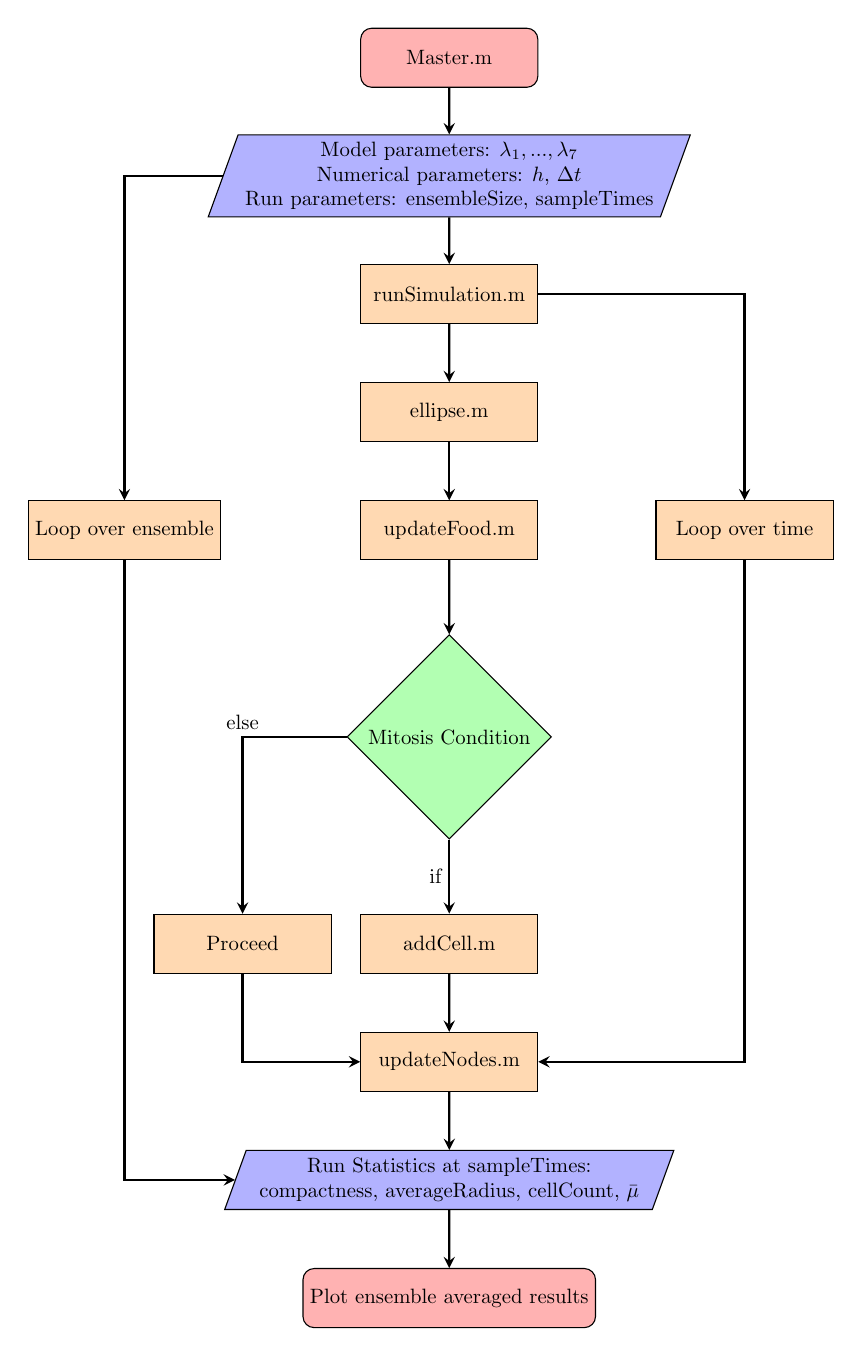
\begin{tikzpicture}[every text node part/.style={align=center}, 
                    node distance=2cm]


    \begin{scope}[scale=0.75,transform shape]
    \node (start) [startstop] {\codeword{Master.m}};
    \node (in1) [io, below of=start] { Model parameters: $\lambda_1, ... , \lambda_7$ \\
                                       Numerical parameters: $h$, $\Delta t$ \\
                                       Run parameters: \codeword{ensembleSize}, \codeword{sampleTimes}};
    \node (pro1) [process, below of=in1] {\codeword{runSimulation.m}};
    \node (pro2) [process, below of=pro1] {\codeword{ellipse.m}};
    \node (pro3) [process, below of=pro2] {\codeword{updateFood.m}};
    \node (dec1) [decision, below of=pro3, yshift=-1.5cm] {Mitosis Condition};
    \node (pro4) [process, below of=dec1, yshift=-1.5cm] {\codeword{addCell.m}};
    \node (proNothing) [process, left of=pro4, xshift=-1.5cm] {Proceed};
    \node (pro5) [process, below of=pro4] {\codeword{updateNodes.m}};
    %\node (pro5) [process, right of=dec1, xshift=2cm] {Process 2b};
    \node (out1) [io, below of=pro5] {Run Statistics at \codeword{sampleTimes}: \\
                                      \codeword{compactness},
                                      \codeword{averageRadius},
                                      \codeword{cellCount},
                                      $\bar{\mu}$};
    \node (stop) [startstop, below of=out1] {Plot ensemble averaged results};
    \node (for) [process, left of=pro3, xshift=-3.5cm] {Loop over ensemble};
    \node (forTime) [process, right of=pro3,  xshift=3.0cm] {Loop over time};

    \draw [arrow] (start) -- (in1);
    \draw [arrow] (in1) -- (pro1);
    \draw [arrow] (pro1) -- (pro2);
    \draw [arrow] (pro2) -- (pro3);
    \draw [arrow] (pro3) -- (dec1);
    \draw [arrow] (dec1) -| node[anchor=south]{else} (proNothing);
    \draw [arrow] (proNothing) |- node[anchor=south]{} (pro5);
    \draw [arrow] (dec1) -- node[anchor=east]{if}(pro4);
    \draw [arrow] (pro4) -- (pro5);
    \draw [arrow] (pro5) -- (out1);
    \draw [arrow] (out1) -- (stop);
    \draw [arrow] (in1) -| node[anchor=south]{} (for);
    \draw [arrow] (for)  |- node[anchor=south]{} (out1);
    \draw [arrow] (pro1)  -| node[anchor=south]{} (forTime);
    \draw [arrow] (forTime)  |- node[anchor=south]{} (pro5);
    
    %\draw [arrow] (pro2a) -- (out1);
    %\draw [arrow] (out1) -- (stop);

    \end{scope}
\end{tikzpicture}
\caption{A flow chart of \textbf{CellColonySimulator} software package in MATLAB. }
\label{fig:softwareFlowChart}
\end{figure}

\newpage





\section{Statistics from the model}
The model developed thus far is a numerical framwork for simulating growing cell colonies.
There is an element of randomness in the model: when two nodes are dislodged from the 
same point there is initially no preferred direction to move in so one must be chosen randomly
before other forces can take effect. For this reason, every seperate run of the model 
starting with identical initial conditions will look very different after time has passed. 
It is expected however that some ``averaged''
quantity will stabilise so long as the model is simulated over a fairly large number of runs.
Seperate runs of the model belong to a set called an ensemble.
We will start with a relatively straightforward metric, the number of cells at time
$T = 500$ steps.
\\

A fully grown colony will in general not be perfectly circular in shape.
 In order to measure the roundness of the colony we use the compactness metric used for 
 roundness in image processing (quote Kai use of this metric)
\begin{equation}
  C = \frac{P^2}{4 \pi A},
\end{equation}
where $C \in [1, \infty)$ is $1$ for a circle and can get to large numbers for 
highly branching shapes, $A$ is the colony area, and $P$ is the colony perimeter. 
Both of these are calculated from the formula for the microscopic cell
density which is always given by when $f(x,y,t)$ changes sign. A black and white image 
is produced at each time step using Matlab's function \codeword{bwboundaries} as per
Kai's suggestion. The area then is given by summing up the grid squares that are
inside the implicit shape givcen by $f$ and multiplying by $h^2$. The perimeter
is got by using \codeword{bwboundaries}, which outputs an array of points on the boundary
from which the Euclidean distance between neighbouring points is found and then summed over.
\begin{figure}[!htb]
    \centering
    \includegraphics[width=\textwidth]{chapter1/figures/compareCompactness.pdf}
    \caption{A comparsion of high and low compactness}
    \label{fig:compatness_comparison}
\end{figure}

\newpage

\begin{figure}[!htb] %Change this to [p] maybe ?
    \centering
    \includegraphics[width= 0.7\textwidth]{
        chapter2/figures/t_all__L1_0o10_L2_1o00_L3_1o00_L4_0o50_L5_1o00_L6_0o50_L7_1o00.pdf}
    \caption{A cell colony with parameter values given by
             $\lambda_1 = 0.1$,  
             $\lambda_2 = 1.0$, 
             $\lambda_3 = 1.0$, 
             $\lambda_4 = 0.5$, 
             $\lambda_5 = 1.0$, 
             $\lambda_6 = 0.5$, 
             $\lambda_7 = 1.0$. 
             On the left we have the biomass field, the nutrient field is on the right.}
    \label{fig: sdsd}
\end{figure}


\newpage


\begin{figure}[!htb] %Change this to [p] maybe ?
    \centering
    \includegraphics[width= 0.7\textwidth]{
        chapter2/figures/t_all_L1_0o10_L2_5o00_L3_1o00_L4_0o50_L5_1o00_L6_2o00_L7_0o50.pdf}
    \caption{A cell colony with parameter values given by
             $\lambda_1 = 0.1$,  
             $\lambda_2 = 5.0$, 
             $\lambda_3 = 1.0$, 
             $\lambda_4 = 0.5$, 
             $\lambda_5 = 1.0$, 
             $\lambda_6 = 2.0$, 
             $\lambda_7 = 0.5$. 
             Biomass on left and nutrient field on the right.}
    \label{fig: sdsd}
\end{figure}

\newpage

\begin{figure}[!htb] %Change this to [p] maybe ?
    \centering
    \includegraphics[width= 0.7\textwidth]{
        chapter2/figures/t_all__L1_0o10_L2_5o00_L3_1o00_L4_0o50_L5_1o00_L6_0o40_L7_0o60.pdf}
    \caption{A cell colony with parameter values given by
             $\lambda_1 = 0.1$,  
             $\lambda_2 = 5.0$, 
             $\lambda_3 = 1.0$, 
             $\lambda_4 = 0.5$, 
             $\lambda_5 = 1.0$, 
             $\lambda_6 = 0.4$, 
             $\lambda_7 = 0.6$. 
             Biomass on left and nutrient field on the right.}
    \label{fig: sdsd}
\end{figure}

\begin{figure}[!htb] %Change this to [p] maybe ?
    \centering
    \includegraphics[width= 0.7\textwidth]{
        chapter2/figures/t_all__L1_0o10_L2_5o00_L3_1o00_L4_0o50_L5_1o00_L6_2o00_L7_0o60.pdf}
    \caption{A cell colony with parameter values given by
             $\lambda_1 = 0.1$,  
             $\lambda_2 = 5.0$, 
             $\lambda_3 = 1.0$, 
             $\lambda_4 = 0.5$, 
             $\lambda_5 = 1.0$, 
             $\lambda_6 = 2.0$, 
             $\lambda_7 = 0.6$. 
             Biomass on left and nutrient field on the right.}
    \label{fig: sdsd}
\end{figure}




\begin{figure}[!htb] %Change this to [p] maybe ?
    \centering
    \includegraphics[width= 1\textwidth]{
        chapter2/figures/SpecificGrowthRatePlot.png}
    \caption{The colony average specific growth rate for different values of $\lambda_5$
                is measured and plotted over time for ensemble size $1$. The rest of the parameters 
                took the values:
                $\lambda_1 = 0.1$,  
                $\lambda_2 = 1.0$, 
                $\lambda_3 = 1.0$, 
                $\lambda_4 = 1.0$, 
                $\lambda_5$ (variable), 
                $\lambda_6 = 0.5$, 
                $\lambda_7 = 0.7$.
                Remarkably, when $\lambda_5 \geq 5.0$ there is an interesting dynamic that 
                occurs based on the compettition between nutrient consumption rate ($\lambda_6$)
                and the mobility ($\lambda_5$). For small values of mobility,
                the cells are not able to move enough into areas where the nutrient has not 
                decayed.}
    \label{fig:ColonySimulationNutrientFieldN210}
    \end{figure}










\section{ Fast computational software in MATLAB }
The software developed for the computational modelling is recquired
to be fast, accurate and easy to understand.






    








\chapter{Numerical experiments and simulation results}


\begin{figure}[!htb] %Change this to [p] maybe ?
    \centering
    \includegraphics[width= 0.7\textwidth]{
        chapter3/figures/t_all_L1_0o10_L2_5o00_L3_5o00_L4_0o50_L5_1o00_L6_3o00_L7_0o50.pdf}
    \caption{A cell colony with parameter values given by
             $\lambda_1 = 0.1$,  
             $\lambda_2 = 5.0$, 
             $\lambda_3 = 5.0$, 
             $\lambda_4 = 0.5$, 
             $\lambda_5 = 1.0$, 
             $\lambda_6 = 3.0$, 
             $\lambda_7 = 0.5$. 
             On the left we have the biomass field, the nutrient field is on the right.}
    \label{fig: sdsd}
\end{figure}

\begin{figure}[!htb] %Change this to [p] maybe ?
    \centering
    \includegraphics[width= 0.7\textwidth]{
        chapter3/figures/t_all_L1_0o10_L2_5o00_L3_5o00_L4_0o50_L5_0o10_L6_0o70_L7_0o73.pdf}
    \caption{A cell colony with parameter values given by
             $\lambda_1 = 0.1$,  
             $\lambda_2 = 5.0$, 
             $\lambda_3 = 5.0$, 
             $\lambda_4 = 0.5$, 
             $\lambda_5 = 0.1$, 
             $\lambda_6 = 0.7$, 
             $\lambda_7 = 0.73$. 
             On the left we have the biomass field, the nutrient field is on the right. 
             The aspect ratio is $\lambda_7 = 5.5/7.5 = 0.73$.}
    \label{fig: sdsd}
\end{figure}

\begin{figure}[!htb] 
    \centering
    \includegraphics[width= 0.7\textwidth]{
        chapter3/figures/t_all_L1_0o10_L2_5o00_L3_5o00_L4_0o50_L5_1o20_L6_0o70_L7_0o60.pdf}
    \caption{A cell colony with parameter values given by
             $\lambda_1 = 0.1$,  
             $\lambda_2 = 5.0$, 
             $\lambda_3 = 5.0$, 
             $\lambda_4 = 0.5$, 
             $\lambda_5 = 1.2$, 
             $\lambda_6 = 0.7$, 
             $\lambda_7 = 0.6$. 
             Biomass on left and nutrient field on the right.}
    \label{fig: sdsd}
\end{figure}

\begin{figure}[!htb] %Change this to [p] maybe ?
    \centering
    \includegraphics[width= 0.7\textwidth]{
        chapter3/figures/t_all_L1_0o10_L2_5o00_L3_5o00_L4_0o50_L5_1o60_L6_0o90_L7_0o95.pdf}
    \caption{A cell colony with parameter values given by
             $\lambda_1 = 0.1$,  
             $\lambda_2 = 5.0$, 
             $\lambda_3 = 5.0$, 
             $\lambda_4 = 0.5$, 
             $\lambda_5 = 1.6$, 
             $\lambda_6 = 0.9$, 
             $\lambda_7 = 0.95$. 
             Biomass on left and nutrient field on the right.}
    \label{fig: sdsd}
\end{figure}

\begin{figure}[!htb] %Change this to [p] maybe ?
    \centering
    \includegraphics[width= 0.7\textwidth]{
        chapter3/figures/t_all_L1_0o10_L2_5o00_L3_5o00_L4_0o50_L5_1o60_L6_0o70_L7_0o50.pdf}
    \caption{A cell colony with parameter values given by
             $\lambda_1 = 0.1$,  
             $\lambda_2 = 5.0$, 
             $\lambda_3 = 5.0$, 
             $\lambda_4 = 0.5$, 
             $\lambda_5 = 1.6$, 
             $\lambda_6 = 0.7$, 
             $\lambda_7 = 0.5$. 
             Biomass on left and nutrient field on the right.}
    \label{fig: sdsd}
\end{figure}

\begin{figure}[!htb]
    \centering
    \includegraphics[width= \textwidth]{
        chapter3/figures/Comp_all_ar_EnsembleSize_6o0_L1_0o10_L2_5o00_L3_5o00_L4_0o50_L5_1o00_L6_1o00_L7_0o40.pdf}
    \caption{The colony compactness and growth rate for 
             $\lambda_1 = 0.1$,  
             $\lambda_2 = 5.0$, 
             $\lambda_3 = 5.0$, 
             $\lambda_4 = 0.5$, 
             $\lambda_5 = 1.0$, 
             $\lambda_6 = 1.0$, 
             $\lambda_7$ variable and an ensemble size of $6$.}
    \label{fig: sdsd}
\end{figure}

\begin{figure}[!htb] %Change this to [p] maybe ?
    \centering
    \includegraphics[width= \textwidth]{
        chapter3/figures/Comp_average_actness_EnsembleSize_6o0_L1_0o10_L2_5o00_L3_5o00_L4_0o50_L5_1o00_L6_1o00_L7_0o40.pdf}
    \caption{The average colony compactness for
             $\lambda_1 = 0.1$,  
             $\lambda_2 = 5.0$, 
             $\lambda_3 = 5.0$, 
             $\lambda_4 = 0.5$, 
             $\lambda_5 = 1.0$, 
             $\lambda_6 = 1.0$, 
             $\lambda_7 = 0.4, 0.5, 0.7, 1.0$ and an ensemble size of $6$.}
    \label{fig: sdsd}
\end{figure}

\begin{figure}[!htb] %Change this to [p] maybe ?
    \centering
    \includegraphics[width= \textwidth]{
        chapter3/figures/Inset_L1_0o10_L2_5o00_L3_5o00_L4_0o50_L5_1o00_L6_1o00_L7_1o00.pdf}
    \caption{Compactness for ensemble instance $e = 1$ and 
             $\lambda_1 = 0.1$,  
             $\lambda_2 = 5.0$, 
             $\lambda_3 = 5.0$, 
             $\lambda_4 = 0.5$, 
             $\lambda_5 = 1.0$, 
             $\lambda_6 = 1.0$, 
             $\lambda_7 = 1.0$. The inset plots show the biomass at three times for comparison 
             with compactness.}
    \label{fig: sdsd}
\end{figure}

\begin{figure}[!htb] %Change this to [p] maybe ?
    \centering
    \includegraphics[width= \textwidth]{
        chapter3/figures/Inset_L1_0o10_L2_5o00_L3_5o00_L4_0o50_L5_1o00_L6_1o00_L7_0o50.pdf}
    \caption{Compactness for ensemble instance $e = 1$ and 
             $\lambda_1 = 0.1$,  
             $\lambda_2 = 5.0$, 
             $\lambda_3 = 5.0$, 
             $\lambda_4 = 0.5$, 
             $\lambda_5 = 1.0$, 
             $\lambda_6 = 1.0$, 
             $\lambda_7 = 0.5$. The inset plots show the biomass at three times for comparison 
             with compactness.}
    \label{fig: sdsd}
\end{figure}


\begin{figure}[!htb] %Change this to [p] maybe ?
    \centering
    \includegraphics[width= \textwidth]{
        chapter3/figures/Inset_L1_0o10_L2_5o00_L3_5o00_L4_0o50_L5_5o00_L6_1o00_L7_0o70.pdf}
    \caption{Specific growth rate $\mu(t)$ for ensemble instance $e = 1$ and 
             $\lambda_1 = 0.1$,  
             $\lambda_2 = 5.0$, 
             $\lambda_3 = 5.0$, 
             $\lambda_4 = 0.5$, 
             $\lambda_5 = 5.0$, 
             $\lambda_6 = 1.0$, 
             $\lambda_7 = 0.7$.}
    \label{fig: sdsd}
\end{figure}

\begin{figure}[!htb] %Change this to [p] maybe ?
    \centering
    \includegraphics[width= \textwidth]{
        chapter3/figures/Inset_L1_0o10_L2_5o00_L3_5o00_L4_0o50_L5_0o10_L6_1o00_L7_0o70.pdf}
    \caption{Specific growth rate $\mu(t)$ for ensemble instance $e = 1$ and 
             $\lambda_1 = 0.1$,  
             $\lambda_2 = 5.0$, 
             $\lambda_3 = 5.0$, 
             $\lambda_4 = 0.5$, 
             $\lambda_5 = 0.1$, 
             $\lambda_6 = 1.0$, 
             $\lambda_7 = 0.7$.}
    \label{fig: sdsd}
\end{figure}

\begin{figure}[!htb] %Change this to [p] maybe ?
    \centering
    \includegraphics[width= \textwidth]{
        chapter3/figures/Comp_all_ar_EnsembleSize_6o0_L1_0o10_L2_5o00_L3_5o00_L4_0o50_L5_0o10_L6_1o00_L7_0o70.pdf}
    \caption{Compactness $C(t)$ and specific growth rate $\mu(t)$ for 
             $\lambda_1 = 0.1$,  
             $\lambda_2 = 5.0$, 
             $\lambda_3 = 5.0$, 
             $\lambda_4 = 0.5$, 
             $\lambda_5 = 0.1, 1.0, 2.5, 5.0$, 
             $\lambda_6 = 1.0$, 
             $\lambda_7 = 0.7$, and an ensemble of size $6$. Note that the bottom panels 
             could only be simulated to $t = 20$ hours due to GPU out-of-memory issues.}
    \label{fig: sdsd}
\end{figure}

\begin{figure}[!htb] %Change this to [p] maybe ?
    \centering
    \includegraphics[width= \textwidth]{
        chapter3/figures/Average_mu_EnsembleSize_6o0_L1_0o10_L2_5o00_L3_5o00_L4_0o50_L5_0o10_L6_1o00_L7_0o70.pdf}
    \caption{Average growth rate $\mu(t)$ for 
             $\lambda_1 = 0.1$,  
             $\lambda_2 = 5.0$, 
             $\lambda_3 = 5.0$, 
             $\lambda_4 = 0.5$, 
             $\lambda_5 = 0.1, 1.0, 2.5, 5.0$, 
             $\lambda_6 = 1.0$, 
             $\lambda_7 = 0.7$, and an ensemble of size $6$. Note the plot 
             for $\lambda_5 = 5.0$ could not be completed on the aviliable hardware
             due to GPU out-of-memory.}
    \label{fig: sdsd}
\end{figure}


\conclusions
The components of this thesis when considered individually
are adapted from previous mathematical 
modelling, sometimes in biology, sometimes not. The value of 
what has been done emerges from the interplay of the elements
\begin{enumerate}
    \item A PDE nutrient field,
    \item An overdamped and growing spring network,
    \item A cell colony given as a level-section of a polynomial,
\end{enumerate}
all of which I feel were necessary for the model's overall 
synthesis to occur. I by no means believe 
that even a small proportion of the total causes and effects
have been accounted for in regard to baker's yeast proliferation 
in nutrient-poor conditions. But it is my hope 
that new model \textit{triple-points} or even \textit{multi-stable symbolic states} 
can be sought after in future 
studies.
\\

Qualitatively different types of models, when coupled
in this attentive way can give rise to new dynamics not found in 
any singular model. That being said, 
the process of learning and tending to more models than one can be
laborious, if not grounded in some sort of overarching 
framework, even if that framework is to disappear 
when the total project emerges.
\\

\textit{A word on my own working process.}
The openness to testing different models without 
the promise of intellectual refuge in one prior form, came 
from my conviction that \textit{life itself} is irreducible
and heterogenous. Our mathematical models sometimes reflect 
this truth (that I have come to understand through struggle, 
hurt and loneliness), and sometimes 
they do not. In that sense, this thesis is a 
\textit{personal reckoning} with the very structuring 
force of our own assumptions. But there are other 
forces at play aswell.
\\

The pressure of scientific tradition was a necessary 
influence on my project, and so was 
my own opposing reaction to its reductionist tendancies.
Without these forces this project would not have 
branched out into what it became. Since 
I too am a living being whose cells 
are in constant interaction with the environment, 
it was necessary to bring my own subjectivity
into this tango of symbols.
\\

In classical mechanics, forces are vectors that 
are summed to give the net force. What we have 
come to forget is that individual forces themselves
could have different mathematical structures associated 
to them. There may be more natural or ergonomic 
formalisms associated to each force. 
The dirrect approach then, is to consider 
``force formalisms" that allow for designed trajectories.
\\

It seems, ``change how you look at it, and you will see something 
different,'' is a dismissal of form. That is not the case. 
There is a rich history of mathematics that studies 
subjectivity directly, but you can only see that if you sit with 
it for long enough. Mathematics is wedded to form and form 
is about perception.
\\

Ironically then, for an applied mathematics thesis grounded 
in the observation of an organism like \textit{S. cerevisiae},
this work is truly endebted to what I imagine 
subjects \textit{topology}, \textit{geometry}, and 
\textit{algebra} to be like. I have studied 
these topics very haphazardly and hope to refine my 
understanding over the next few years.



\begin{appendices}
\renewcommand{\thesection}{A.\arabic{section}}
\section{Collocation algorithm with mask matrices}
Each cell indexed $j \in \{1, \ldots N\}$ has five pieces of data which are enough to define globally the 
SDF of the cell, namely, the center coordinates $(x_j,y_j)$, the angle of orientation $\theta_j$, 
and the semi axes dimensions $a_j, b_j$. Each piece of data will be a function of time $t$. For 
the purpose of simplicity, we model each cell as two point masses $m_1 = m_2 = m$ connected by a spring 
with stiffness $K$. The point masses are located at $\vb{r}_j^{(1)}$ and $\vb{r}_j^{(2)}$ inside the ellipse 
along the major axis and symmetrically about the ellipse center. This means that the center is given by 
\begin{equation*}
    \vb{x}_j = \frac{1}{2} \left(\vb{r}_j^{(1)} + \vb{r}_j^{(2)}\right).
\end{equation*}
Fixing the semi-minor axis $b_j$, we give the semi-major axis $a_j$ by 
\begin{equation*}
    a_j = a_0||\vb{r}_j^{(1)} - \vb{r}_j^{(2)}||.
\end{equation*}
We extract the orientation angle using a two argument inverse tangent function,
\begin{equation*}
    \theta_j = \arctan(y_j^{(2)} - y_j^{(1)},x_j^{(2)} - x_j^{(1)} )
\end{equation*}

When the number of cells is fixed, the colony dynamics is modelled
using first order EOMs with two primary forces: intracellular spring force and
and intercellular contact force to void overlap. We take the assumption that 
many authors make (include reference here) which is that inertia is negligible
due to drag effects (more on this). That is the velocity is directly
proportional to the force
\begin{equation*}
\vb{v}_j^{(i)} = \frac{1}{\eta} \vb{F}_j^{(i)},
\end{equation*}
where $i \in \{1,2\}$ and $j \in \{1, \ldots, N\}$ where $\eta$ is an expression for
the drag and $\vb{F}_j^{(i)}$ is the sum of the forces acting on the $i$-th particle of
the $j$-th cell. Overall, the simulation will be begun with $V$ vertices where $V$ is a
positive power of $2$. We map from local indices $(i,j)$ to a global index $n$ using
\begin{equation*}
    n = 2(j-1) +i,
\end{equation*}
which is called ``row major order''. We then flatten the list of $x$-coordinates and 
$y$-coordinates into one state vector $\vb{X}(t)$ given by
\begin{equation*}
    \vb{X}(t) = [x_1(t), \ldots, x_V(t), y_1(t), \ldots, y_V(t)]^T,
\end{equation*}
where $(x_n,y_n)$ is the coordinate of the $n$-th vertex for $n \in \{1,\ldots,V\}$.
Note that the change in the number of cells is simulated by removing constraints
between the vertices. At the beginning of the simulation $x_1 = \cdots = x_V$ and
$y_1 = \cdots = y_V$. The first order ordinary differential equation is phrased
in terms of a mass matrix and a force function,
\begin{equation*}
    M(t,\vb{X})\frac{d \vb{X} (t)}{dt} = f(t,\vb{X})
\end{equation*}
We start by considering the spring force acting on the $n$-th particle due to the $m$-th 
particle given $n$ and $m$ are connected by springs. This is given by $\vb{F}_{nm}^{\textrm{spring}}$ as
\begin{equation*}
    \vb{F}_{nm}^{\textrm{spring}} = 
    K(|| \vb{x}_m - \vb{x}_n|| - L_{nm}) \frac{\vb{x}_m - \vb{x}_n}{|| \vb{x}_m - \vb{x}_n||},
\end{equation*}
where $K$ is a spring constant meant to represent cell elasticity, and $L_{nm}$ is the nominal length
of the spring connecting them. There are three situations regarding edge between vertex $n$ and $m$:
either they are connected by a spring with $L_{nm}>0$, they are collocated by an equality constraint
or they are disconnected. If the two masses are collocated by an equality constraint, then the 
spring force is undefined so we must omit this. We must also omit the contact force because this 
has no sense for collocated vertices. The contact force between two disconnected vertices is given as
\begin{equation*}
    \vb{F}_{nm}^{\textrm{contact}} =
    \begin{cases} 
        C\frac{\vb{x}_m - \vb{x}_n}{|| \vb{x}_m - \vb{x}_n||}, \ \textrm{if} \ || \vb{x}_m - \vb{x}_n|| \leq d \\
        \vb{0}, \ \textrm{if} \ || \vb{x}_m - \vb{x}_n|| > d,
    \end{cases}
\end{equation*}
which is used to ensure that vertices do not overlap past a threshold distance $d$. In terms of the 
connectivity, we can encode the fact that two vertices are connected (by a spring) in an adjacency matrix
$A_{nm}$ which is equal to $1$ if they are connected and $0$ otherwise. We also introduce a second matrix
$B_{nm}$ which represents when two vertices are disconnected, i.e., $B_{nm} = 1 - A_{nm}$. A third matrix 
is introduced for collocation $C_{nm} = 1$ if $n \neq m$ and $n$ and $m$ are collocated and $0$ otherwise.
This matrix (in fact $\tilde{C}_{nm} = \sim C_{nm}$) will be used as a logical mask to filter out 
\codeword{nan} values from the force matrices. 
\\
\\
We can think of the forces (whether elastic or contact) as pairs of matrices $(F_x)_{nm}^{\textrm{spring}}$ and 
$(F_y)_{nm}^{\textrm{spring}}$ and similarly for the contact forces. We construct the $x$-component of 
the overall force vector
\begin{equation*}
    (f_x)_n = 
    \sum_{m=1}^V((F_x)^{\textrm{spring}}(A {\&}  \tilde{C}))_{nm} + 
    \sum_{m=1}^V((F_x)^{\textrm{contact}}( B  {\&}  \tilde{C}))_{nm} ,
\end{equation*}
where $A  {\&}  \tilde{C}$ are mask matrices that ensure both $A$ and not $C$ are satisfied. Similarly for the 
$y$-component,
\begin{equation*}
    (f_y)_n = 
    \sum_{m=1}^V((F_y)^{\textrm{spring}}(A {\&}  \tilde{C}))_{nm} + 
    \sum_{m=1}^V((F_y)^{\textrm{contact}}( B  {\&}  \tilde{C}))_{nm}.
\end{equation*}
The question remains: how are the mask matrices $A$, $B$ and $C$ made to change over time? Here we will do
a small illustrative example with $N=4$ cells and $V=2N = 8$ vertices. 
\\
\\
Initially all the vertices will be
collocated at the same position $(x_0,y_0)$. This means that the force vector should come out to zero because
we essentially have one particle not interacting with anything. Let us check that $A  {\&}  \tilde{C}$ and 
$B  {\&}  \tilde{C}$ both vanish. $C$ is given directly as a matrix of all ones, which says that each vertex
is constrained to every other vertex. Thus $\tilde{C} = O$ where $O$ is a  $8 \times 8$ zero matrix. 
Initially, say $A = O$ (the zero matrix) because there are no springs. Note that this immediately says that 
$B$ is a matrix of all ones. In any case, both $A  {\&}  \tilde{C} = B  {\&}  \tilde{C} = O$.
\\
\\
At some point, the effectively single particle starts growing away from its initial position. This is 
achieved by parcelling half of the vertices into one set of collocated points, and the other half
into another set of collocated points. Programmatically, we select half of the points
and translate them to a random nearby position to $(x_0,y_0)$ and modify the $C$ matrix to remove
the constraints between the first and second set,
\begin{equation*}
    C = 
    \begin{bmatrix}
    1 & 1 & 1 & 1 & 0 & 0 & 0 & 0 \\
    1 & 1 & 1 & 1 & 0 & 0 & 0 & 0 \\
    1 & 1 & 1 & 1 & 0 & 0 & 0 & 0 \\
    1 & 1 & 1 & 1 & 0 & 0 & 0 & 0 \\
    0 & 0 & 0 & 0 & 1 & 1 & 1 & 1 \\
    0 & 0 & 0 & 0 & 1 & 1 & 1 & 1 \\
    0 & 0 & 0 & 0 & 1 & 1 & 1 & 1 \\
    0 & 0 & 0 & 0 & 1 & 1 & 1 & 1 
    \end{bmatrix}
\end{equation*}
At this point, we should also set the nominal length of the springs as $L_0$ and the corresponding
matrix of lengths $L_{mn} = L_0$ (the constant matrix with value $L_0$). As it turns out, the action
of the spring pressing the vertices apart will model the geometric growth of each elliptical cell.
The $A$ matrix will be given by
\begin{equation*}
    A = 
    \begin{bmatrix}
    0 & 0 & 0 & 0 & 1 & 0 & 0 & 0 \\
    0 & 0 & 0 & 0 & 0 & 1 & 0 & 0 \\
    0 & 0 & 0 & 0 & 0 & 0 & 1 & 0 \\
    0 & 0 & 0 & 0 & 0 & 0 & 0 & 1 \\
    1 & 0 & 0 & 0 & 0 & 0 & 0 & 0 \\
    0 & 1 & 0 & 0 & 0 & 0 & 0 & 0 \\
    0 & 0 & 1 & 0 & 0 & 0 & 0 & 0 \\
    0 & 0 & 0 & 1 & 0 & 0 & 0 & 0 
    \end{bmatrix}
\end{equation*}
Now let's suppose that the vertices in one set undergo another mitosis event, splitting half of the particles
off into a third set. The new $C$ matrix, called $C'$ must reflect this change. We call 
$C(\alpha_1, \ldots, \alpha_M) = \textrm{diag}(\vb{1}_{V/2^{\alpha_1}}, \ldots,\vb{1}_{V/2^{\alpha_M}} )$ where $\vb{1}_{V/2^{\alpha_q}}$
is an all $1$'s matrix of dimension $V/2^{\alpha_q} \times V/2^{\alpha_q}$ where $q$ indexes over the powers 
of two and represents the accumulation of division events. During a mitosis event in which the $\alpha_q$-th vertex set
splits, $C(\alpha_1, \alpha_2, \ldots, \alpha_M) \rightarrow 
C(\alpha_1, \ldots, \alpha_q+1,\alpha_q+1 , \ldots\alpha_M)$. In other words, the $\alpha_q$-th matrix splits into
two matrices of half the size. In our $8 \times 8$ case, in which we divide the second vertex set, this results
in the following
\begin{equation*}
    C = 
    \begin{bmatrix}
    1 & 1 & 1 & 1 & 0 & 0 & 0 & 0 \\
    1 & 1 & 1 & 1 & 0 & 0 & 0 & 0 \\
    1 & 1 & 1 & 1 & 0 & 0 & 0 & 0 \\
    1 & 1 & 1 & 1 & 0 & 0 & 0 & 0 \\
    0 & 0 & 0 & 0 & 1 & 1 & 0 & 0 \\
    0 & 0 & 0 & 0 & 1 & 1 & 0 & 0 \\
    0 & 0 & 0 & 0 & 0 & 0 & 1 & 1 \\
    0 & 0 & 0 & 0 & 0 & 0 & 1 & 1 
    \end{bmatrix}
\end{equation*}
The new matrix $A$ is got by adding a connections between the left over smaller matrices, which
is best understood by visualising the matrix as
\begin{equation*}
    A = 
    \begin{bmatrix}
    0 & 0 & 0 & 0 & 1 & 0 & 0 & 0 \\
    0 & 0 & 0 & 0 & 0 & 1 & 0 & 0 \\
    0 & 0 & 0 & 0 & 0 & 0 & 1 & 0 \\
    0 & 0 & 0 & 0 & 0 & 0 & 0 & 1 \\
    1 & 0 & 0 & 0 & 0 & 0 & 1 & 0 \\
    0 & 1 & 0 & 0 & 0 & 0 & 0 & 1 \\
    0 & 0 & 1 & 0 & 1 & 0 & 0 & 0 \\
    0 & 0 & 0 & 1 & 0 & 1 & 0 & 0 
    \end{bmatrix}
\end{equation*}
Taking another division event on the second block, we get
\begin{equation*}
    C = 
    \begin{bmatrix}
    1 & 1 & 1 & 1 & 0 & 0 & 0 & 0 \\
    1 & 1 & 1 & 1 & 0 & 0 & 0 & 0 \\
    1 & 1 & 1 & 1 & 0 & 0 & 0 & 0 \\
    1 & 1 & 1 & 1 & 0 & 0 & 0 & 0 \\
    0 & 0 & 0 & 0 & 1 & 0 & 0 & 0 \\
    0 & 0 & 0 & 0 & 0 & 1 & 0 & 0 \\
    0 & 0 & 0 & 0 & 0 & 0 & 1 & 1 \\
    0 & 0 & 0 & 0 & 0 & 0 & 1 & 1 
    \end{bmatrix}
\end{equation*}
and 
\begin{equation*}
    A = 
    \begin{bmatrix}
    0 & 0 & 0 & 0 & 1 & 0 & 0 & 0 \\
    0 & 0 & 0 & 0 & 0 & 1 & 0 & 0 \\
    0 & 0 & 0 & 0 & 0 & 0 & 1 & 0 \\
    0 & 0 & 0 & 0 & 0 & 0 & 0 & 1 \\
    1 & 0 & 0 & 0 & 0 & 1 & 1 & 0 \\
    0 & 1 & 0 & 0 & 1 & 0 & 0 & 1 \\
    0 & 0 & 1 & 0 & 1 & 0 & 0 & 0 \\
    0 & 0 & 0 & 1 & 0 & 1 & 0 & 0 
    \end{bmatrix}
\end{equation*}

\newpage


\section{Cell-cell collisions with constrained dynamics} \label{collisionModel}
Earlier, it was mentioned that the intersection of cells could be found by taking a smoothmax. To find the overlapping area
the sum of the grid points in the intersection can be taken and then multiplied by the grid square area $h_x h_y$. Whilst
it is more or less trivial to calculate the overlapping area, ensuring that this area remains zero throughout the simulation
is more involved. We employ the technique explained by \cite{witkin1997introduction} based on constrained
dynamics. The constraint in this case is that the area $C$ remains $0$ for all times,
\begin{equation}
    C(\vb{q}) = 0,
\end{equation}
where $\vb{q}$ is the concatenated state vector of the system. One should be aware that, if we have multiple colonies, it will
be required to have pairwise constraints forcing no overlap between each of the constitiuent colonies. For the purpose of simplicity
our state vector $\vb{q}$ will just take into account position and orientation and not size of cells. Later on, this will be generalized.
Therefore $\vb{q}$ is produced by concatenating over $\vb{q}_j$ into one $3N \times 1$ column vector, where
\begin{equation}
\vb{q}_j = \begin{bmatrix}
                x_j \\
                y_j \\
                \theta_j
            \end{bmatrix}.
\end{equation}
Of course, the number of variables per cell can be larger but this comes at a cost in computational time. Recall that the 
intersecting area is secretly a function of the cell state coordinates $\vb{q}_j$ since we are taking a smoothmax of the SDFs 
of each cell. In other words,
\begin{equation*}
f_{\textrm{intersect}}(x,y,\vb{q}) = \textrm{smoothmax}(f_1(x,y,\vb{q}) , \ldots, f_N(x,y,\vb{q}) ),
\end{equation*}

for concreteness, we write out the formula for smoothmax which is the negative smoothmin of the negatives of the SDFs or
\begin{equation*}
    f_{\textrm{intersect}}(x,y,\vb{q}) = -\textrm{smoothmin}(-f_1(x,y,\vb{q}) , \ldots, -f_N(x,y,\vb{q}) ).
\end{equation*}
In full this boils down to,
\begin{equation*}
    f_{\textrm{intersect}}(x,y,\vb{q}) = k \log( \sum_{j=1}^N e^{f_j(x,y,\vb{q})/k}).
\end{equation*}
Now we assume the state is given by five variables for full generality:
\begin{equation}
\vb{q}_j(t) = 
\begin{bmatrix}
    x_j (t) \\
    y_j(t) \\
    \theta_j(t) \\
    b_j(t) \\
    R_j(t)
\end{bmatrix},
\end{equation}
where $b(t)$ is the semi-major axis length and $R_j(t) \in (0,1]$ is the aspect ratio of the elliptical cell so the semi-minor axis is given by $a_j(t) = R_j(t) b_j(t)$. 
Why are we going to the effort to write out $C(\vb{q})$ in full? Because we need to compute the Jacobian of $C(\vb{q})$ with
respect to $\vb{q}$ in order to carry out the constrained dynamics algorithm. The upshot is that smoothmax is differentiable
whereas maximum is not differentiable. 

We define the region in $\mathbb{R}^2$ to integrate over by 
\begin{equation}
    \Omega(\vb{q}) = \{ (x,y) \in \mathbb{R}^2 \ | \ f_{\textrm{intersect}}(x,y,\vb{q}) \leq 0 \},
\end{equation}
so that the area of the overlapping region is simply a two-dimensional integral over $\Omega(\vb{q})$ of $1$,
\begin{equation}
    C(\vb{q}) = \int\int_{\Omega(\vb{q})} dxdy.
\end{equation}
Now we break up the integral into a sum over simply connected components (SCC) so that we can safely apply Leibniz's rule
\begin{equation}
    C(\vb{q}) = \sum_{i \in SCC(\vb{q})}\int\int_{\Omega_i(\vb{q})} dxdy.
\end{equation}
Leibniz's rule tells us how to carry out a total derivative of $\int\int_{\Omega_i(\vb{q})} dxdy$ with respect to $t$ which determines $\vb{q}$. Let's take that total
derivative now to attain
\begin{equation}
   \frac{d}{dt}\int\int_{\Omega_i(\vb{q})} dxdy = \int\int_{\Omega_i(\vb{q})} \pdv{(1)}{t} dxdy + 
   \int_{\partial \Omega_i(\vb{q})} (1) \vb{v}_{\partial \Omega_i(\vb{q})} \cdot \hat{\vb{n}} dl,
\end{equation}
where $\vb{v}_{\partial \Omega_i(\vb{q})}$ is the ``Eulerian'' velocity of the boundary of the $i$-th SCC. All of this can be avoided if we integrate over a smoothstep
which is defined in our region.
\begin{equation}
    C(\vb{q}) = \int\int_{D} \left[ \frac{1}{2} +\frac{1}{2} \tanh{ \left(- \frac{1}{K}f_{\textrm{intersect}}(x,y,\vb{q}) \right)}\right]dxdy,
\end{equation}
where $D$ is the entire domain of the pertri dish.


\begin{equation*}\
\pdv{f_{\textrm{intersect}}(x,y,\vb{q})}{\vb{q}} = \frac{ \sum_{j=1}^N \pdv{f_j(x,y,\vb{q})}{\vb{q}}e^{f_j(x,y,\vb{q})/k}}{ \sum_{j=1}^N e^{f_j(x,y,\vb{q})/k}}.
\end{equation*}
Conveniently, computing the Jacobian, has turned into $N$ problems that are easier to solve individually. Namely computing $\pdv{f_j(\vb{q})}{\vb{q}}$.
This requires us to express the SDF for an ellipse in terms of the query point $(x,y)$, the center of the cell $(x_j,y_j)$, and its orientation $\theta_j$. This
is given in terms of $l_j^-(\vb{q}, x, y)$ and $l_j^+(\vb{q}, x, y)$ which are given in the ellipse formula. We use MATLAB's symbolic toolbox to compute the
ellipse Jacobian $\pdv{f_j(x,y,\vb{q})}{\vb{q}}$ and return a function that can take numerical inputs using \codeword{matlabFunction(J,"File","ellipseJacobian")}.
With that we can compute Jacobian of the constraint using
\begin{equation} 
    \pdv{C(\vb{q})}{\vb{q}} = -\frac{1}{2K} \int \int_D \left[ 1- \tanh[2]( -\frac{f_{\textrm{intersect}}(x,y,\vb{q})}{K}) \right] \pdv{f_{\textrm{intersect}}(x,y,\vb{q})}{\vb{q}} dx dy.
\end{equation}
Now that all the derivatives have been computed analytically, we can carry out the computation of the integral over $x$ and $y$ using a numerical integral in MATLAB.
From now we use $f$ instead of $f_{\textrm{intersect}}$ for brevity, and we pass to index notation, instead expression the $\beta$-th component of $J$ as 
\begin{equation}
J_{\beta} = -\frac{1}{2K} \int \int_D \left[ 1- \tanh[2]( -\frac{f(x,y,\vb{q})}{K}) \right] \pdv{f(x,y,\vb{q})}{q_{\beta}} dx dy.
\end{equation}
For the computation of constraint forces, we need to further compute the total derivative of the Jacobian with respect to time. This turns 
out to be realted to the Hessian matrix of $C(\vb{q})$ (for no explicit time dependence), as 
\begin{equation*}
    \dot{J}_{\beta} = \sum_{\alpha = 1}^{5N} \dot{q}_{\alpha} \frac{\partial^2 C}{ \partial q_{\alpha} \partial q_{\beta}} = \sum_{\alpha = 1}^{5N} \dot{q}_{\alpha} H_{\alpha, \beta},
\end{equation*}
We need to compute how the Hessian of $C$ can be written in terms of the Hessian and Jacobian of $f$.
\begin{equation}
    \frac{\partial^2 C}{ \partial q_{\alpha} \partial q_{\beta}} = \frac{\partial }{\partial q_{\alpha}} J_{\beta}
\end{equation}
Crunching the calculuations we get
\begin{equation}
 \frac{\partial }{\partial q_{\alpha}} J_{\beta} = -\frac{1}{4 K^2} \int \int_D \left[ 1- \tanh[2]( -\frac{f}{K}) \right] \left[\tanh(-\frac{f}{K})\pdv{f}{q_{\alpha}}\pdv{f}{q_{\beta}} + K \frac{\partial^2 f}{ \partial q_{\alpha} \partial q_{\beta}}\right]  dx dy
\end{equation}
Luckily, the Hessian is built into MATLAB's symbolic toolbox, so we can just call \codeword{matlabFunction(H,"File","ellipseHessian")} and the function to compute
the Hessian is saved into our working directory. Note that the function \codeword{ellipseHessian} computes a $5 \times 5 \times N_{\textrm{grid}} \times N_{\textrm{grid}}$ matrix. 
We call it for each cell $j \in \{1, \ldots, N\}$ but recall that for a given value of $\vb{q}$, the Hessian still has $(x,y)$ as free field variables. In order to integrate
the field data, we use the cell-wise Jacobian field $J_{\beta}^j (x,y)$ and the cell-wise Hessian field $H_{\alpha, \beta}^j (x,y)$ to calculate the overall Hessian field for $f$
\begin{equation*}
    \frac{\partial^2 f}{ \partial q_{\alpha} \partial q_{\beta}} = \left(\frac{1}{k}\right) \left[ \frac{\left(\sum_{j=1}^N E_j\right) \left( \sum_{j=1}^N E_j (k H_{\alpha, \beta}^j + J_{\alpha}^j J_{\beta}^j)\right) - \left(\sum_{j=1}^N E_j J_\alpha^j \right) \left(\sum_{j=1}^N E_j J_\beta^j \right)}{\left(\sum_{j=1}^N E_j\right)^2} \right],
\end{equation*}
where $E_j = e^{f_j/k}$ is used for short. To actually compute the overall integrals for $\pdv{C}{q_{\beta}}$ and $\frac{\partial^2 C}{ \partial q_\alpha \partial q_\beta }$
we use MATLAB's \codeword{trapz} function the following way
\begin{lstlisting}[style=Matlab-editor]
    trapz(y_lin,trapz(x_lin,integrandJacobian,3),2);
\end{lstlisting}
or, in the case of the Hessian,
\begin{lstlisting}[style=Matlab-editor]
    trapz(y_lin,trapz(x_lin,integrandHessian,4), 3);
\end{lstlisting}
where the integrand in the Jacobian cas is given by
\begin{equation*}
    F_{\beta}(x,y) = \left(\frac{T^2-1}{2K} \right)\frac{ \sum_{j=1}^N J_\beta^j E_j}{ \sum_{j=1}^N E_j},
\end{equation*}
where $T = \tanh( -\frac{f(x,y,\vb{q})}{K})$ and, in the case of the Hessian
\begin{equation*}
    G_{\alpha, \beta}(x,y) = 
\left(\frac{T^2-1}{4K^2} \right) \left(T \left(\frac{ \sum_{j=1}^N J_\alpha^j E_j}{ \sum_{j=1}^N E_j}\right) \left(\frac{ \sum_{j=1}^N J_\beta^j E_j}{ \sum_{j=1}^N E_j}\right) + K \frac{\partial^2 f}{ \partial q_{\alpha} \partial q_{\beta}} \right),
\end{equation*}
which, after some serious simplification becomes
\begin{equation*}
    G_{\alpha, \beta}(x,y) = \frac{T^2-1}{4Kk \left(\sum_{j=1}^N E_j\right)^2} \sum_{n=1}^N \sum_{m=1}^N E_n E_m \bigg[ \left( \frac{kT-K}{K}\right) J_\alpha^n J_\beta^m +J_\alpha^m J_\beta^m +k H_{\alpha, \beta}^m \bigg]
\end{equation*}
To make things neat we replace $B = \frac{T^2-1}{4K^2}$, $\hat{E} = \sum_{j=1}^N E_j$ and we subsitute the ratio of the smoothstep and smoothmax parameters
$S = K/k$ to attain,
\begin{equation*}
    G_{\alpha, \beta}(x,y) = \frac{B}{\hat{E}^2} \sum_{n=1}^N \sum_{m=1}^N E_n E_m \bigg[   S(k H_{\alpha, \beta}^m +J_\alpha^m J_\beta^m )+ (T-S)J_\alpha^n J_\beta^m\bigg],
\end{equation*}
Thus we can write 
\begin{equation*}
    J_\beta =  \int \int_D F_{\beta}(x,y) dx dy,
\end{equation*}
\begin{equation*}
    \dot{J}_\beta =\sum_{\alpha=1}^{5N}\dot{q}_\alpha \int \int_D G_{\alpha, \beta}(x,y) dx dy,
\end{equation*}
Now we subsitute to obtain the final integral formulae:
\begin{equation*}
    J_\beta =  \int \int_D \frac{B}{\hat{E}S} \sum_{j=1}^N J_\beta^j E_j dx dy,
\end{equation*}
\begin{equation*}
    \dot{J}_\beta = \int \int_D \frac{B}{\hat{E}^2}  \sum_{\alpha=1}^{5N}  \sum_{n=1}^N \sum_{m=1}^N \dot{q}_\alpha E_n E_m \bigg[   S(k H_{\alpha, \beta}^m +J_\alpha^m J_\beta^m )+ (T-S)J_\alpha^n J_\beta^m\bigg] dx dy.
\end{equation*}
We set out to calculate the following scalar $A = JWJ^t$ where $W = M^{-1}$ is the inverse mass matrix of our dynmical system. Note, that since we have 
only one constraint our goal is to solve for one Lagrange multiplier $\lambda$ which is given as 
\begin{equation*}
A \lambda = - \sum_{\beta =1 }^{5N }\dot{J}_\beta \dot{q}_\beta - JWQ -\kappa_s C -\kappa_d \dot{C},
\end{equation*}
Recall $C = \frac{1}{2}\int \int_D (1+T) dx dy$ and $\dot{C} = \sum_{\beta=1}^{5N} \dot{q}_\beta J_\beta$. This means we can write out our equation for $\lambda$ explicitely
\begin{equation*}
    \left( \sum_{\alpha=1}^{5N} \sum_{\beta=1}^{5N} J_\alpha W_{\alpha, \beta} J_\beta \right) \lambda = - \sum_{\beta =1 }^{5N }\dot{J}_\beta \dot{q}_\beta - \sum_{\alpha =1}^{5N} \sum_{\beta =1}^{5N}J_\alpha W_{\alpha,\beta} Q_\beta -\kappa_s \frac{1}{2}\int \int_D (1+T) dx dy -\kappa_d \sum_{\beta=1}^{5N} \dot{q}_\beta J_\beta,
\end{equation*}
Note that its convenient from a computatational point of view to bring the quadriple sum into the integral and then evaluate this using \codeword{trapz}:
\begin{equation*}
    \int \int_D \frac{B}{\hat{E}^2}  \sum_{\alpha=1}^{5N} \sum_{\beta=1}^{5N}  \sum_{n=1}^N \sum_{m=1}^N (\dot{q}_\alpha \dot{q}_\beta E_n E_m )\bigg[   S(k H_{\alpha, \beta}^m +J_\alpha^m J_\beta^m )+ (T-S)J_\alpha^n J_\beta^m\bigg] dx dy.
\end{equation*}
where the term $\dot{q}_\alpha \dot{q}_\beta E_n E_m$ is a $(5N) \times (5N) \times N \times N \times N_{\textrm{grid}} \times N_{\textrm{grid}}$ array.
Now, of course the integral we are after is the following
\begin{equation*}
    I_{\alpha, \beta}^{l,m,n} = \int \int_D \frac{B_l}{E_l^2} (E_n E_m )\bigg[   S(k H_{\alpha, \beta}^m +J_\alpha^m J_\beta^m )+ (T_l-S)J_\alpha^n J_\beta^m\bigg] dx dy.
\end{equation*}
Observing this formula, we can note that $\hat{E}$ has been replaced by $E_l$. This is actually an improvement since $\hat{E}$ was only ever part of the
smoothmax approximation, we replace it by an arbitrary $E_l$ which must be picked prior to evaluating the integral based on the maximum. I have subscripted $B_l$ and $T_l$
similarly as they depend on $E_l$. The main reason for this was due to difficulty in evaluating the integral over a reciprical sum when $N$ was arbitrary. Note that 
if we evaluate this integral symbolically in preprocessing we can essentially divide the amount of computational work by $10^6$ for a $1000 \times 1000$ grid. Even
now, the compute time scales as $N^4$ for $N$ cells. This is still intractable. A significant optimisation can be made when we realise that, from the point of view of a partial
derivative, a cell's SDF is not affected by the coordinates of another cell. Another way to put this is that the Jacobian and Hessian for a given cell $j$
depend only on the attributes of that cell and all the other partial derivatives will vanish. This actually reduces the ammount to compute by a factor of $N^2$ because
we only need to sum over the number of attributes per cell ($N_{\textrm{attrib}} = 5$ in our case) squared. A modern laptop can perform floating point
operations in the order of tens of GFLOPS. Supposing the calculation of $I_{\alpha, \beta}^{l,m,n}$ requires $1000$ floating point operations per $(m,n)$ pair. If we try
to push to $N = 1000$ yeast cells, then we will be looking at a second compute time per time step assuming the PC used operates at $1$ GFLOP. This is fine
for small $N$ but the problem doesn't scale well. In any case, with the current optimisations, we have a tractable simulaton.
\\
It is worth noting that further optimisations can be made if we employ a spatial hash map or a AABB filter which avoids computing matrix elements 
between cells which are not even nearby each other. For example, if cells $3$ and $22$ are further than $d$ apart where $d$ is the pair's maximum cell diameter
then we can set the matrix element $I_{\alpha, \beta}^{l,3,22} =I_{\alpha, \beta}^{l,22,3} = 0$ straight away (Note sure about this). We carry the full computation 
in the test phase and add the filter optimisation later.
\\
\\ 
\end{appendices}

\backmatter
% Add the bibliography to the table of contents
\nocite{*} %remove when you begin to cite things in the main text
\addcontentsline{toc}{chapter}{Bibliography}
\bibliographystyle{apa} % choose whatever style you wish, I don't believe there is a requirement from the university
\bibliography{reference_list} % this is a bibtext reference list. Use a reference manager such a Jabref to maintain your references and save to this directory.


\end{document}

